\documentclass[10pt]{beamer}

\usepackage[utf8]{inputenc}
\usepackage[british]{babel}
\usepackage{color}
%\usepackage{auto-pst-pdf}
\usepackage{pstricks,multido}
\usepackage{graphicx} 
\usepackage{listings,multicol}
\lstdefinelanguage{json}{
  keywords={},
  keywordstyle=\bfseries,
  ndkeywords={},
  ndkeywordstyle=\bfseries,
  sensitive=false,
  comment=[l]{//},
  morecomment=[s]{/*}{*/},
  commentstyle=\ttfamily,
  stringstyle=\ttfamily,
  morestring=[b]',
  morestring=[b]"
}
\usepackage{multirow}
\usepackage{amsfonts}
\usepackage{tabu}
\usepackage{svgcolor}
\usepackage{pst-slpe}
\usepackage{calc}
\usepackage{eurosym}

\newcommand{\ABS}[1]{\left|#1\right|}
\newcommand{\C}[1]{\left[#1\right]}
\newcommand{\MATRIX}[2]{\PA{\begin{array}{#1}#2\end{array}}}
\newcommand{\PA}[1]{\left(#1\right)}
\newcommand{\LL}[1]{\left\{#1\right\}}

\usetheme{Darmstadt}
%\usetheme{Hannover}
%\usetheme{Frankfurt}
%\usetheme{Rochester}
%\usetheme{Copenhagen}

\title{MPCOTool: a tool for optimization and calibration of models}
\author{Javier Burguete}
\institute{Soil and Water Department. EEAD/CSIC}
\date{\today}

\newcommand{\PICTURE}[2]
{
	\begin{figure}[ht]
		\centering
		\begin{picture}(#1)
			#2
		\end{picture}
	\end{figure}
}

\newcommand{\PSPICTURE}[5]
{
	\begin{figure}[ht!]
		\centering
		\pspicture(#1,#2)(#3,#4)
			#5
		\endpspicture
	\end{figure}
}

\newcommand{\FIGURE}[2]
{
	\begin{center}
		\includegraphics[#1]{#2}
	\end{center}
}

\newcommand{\TABLE}[3]
{
	\begin{table}[ht!]
		\centering
		#1
		\tabulinesep=0.9mm
		\begin{tabu}{#2}
			#3
		\end{tabu}
	\end{table}
}

\begin{document}

\begin{frame}
	\titlepage
\end{frame}

\begin{frame}
	\frametitle{Index}
	\tableofcontents
\end{frame}

\section{Introduction}

\begin{frame}
	\begin{itemize}
		\item Models: necessity of empirical paramters
		\item Calibration: fit empirical parameters by optimization
		\item Optimization: minimization of an objective function
	\end{itemize}
\end{frame}

\section{Optimization}

\subsection{Algorithms}

\begin{frame}
	\begin{itemize}
		\item Stochastics
			\begin{itemize}
				\item Brute force
					\begin{itemize}
						\item Sweep
						\item Monte-Carlo
					\end{itemize}
				\item Iteratives
				\item Genetics
			\end{itemize}
		\item Direction search
	\end{itemize}
\end{frame}

\begin{frame}
	\frametitle{Sweep}
\PICTURE{210,200}
{
	\put(20,10){\vector(0,1){180}}
	\put(20,10){\vector(1,0){180}}
	\put(10,190){$y$}
	\put(200,0){$x$}
	\multiput(50,40)(30,0){5}{\qbezier[40](0,0)(0,60)(0,120)}
	\multiput(50,40)(0,30){5}{\qbezier[40](0,0)(60,0)(120,0)}
	\multiput(50,40)(30,0){5}{\multiput(0,0)(0,30){5}{\circle*{2}}}
	\qbezier[10](50,10)(50,25)(50,40)
	\put(40,0){$x_{\min}$}
	\qbezier[10](170,10)(170,25)(170,40)
	\put(160,0){$x_{\max}$}
	\qbezier[10](20,40)(35,40)(50,40)
	\put(0,37){$y_{\min}$}
	\qbezier[10](20,160)(35,160)(50,160)
	\put(0,157){$y_{\max}$}
}
\end{frame}

\begin{frame}
	\frametitle{Monte-Carlo}
\PICTURE{210,200}
{
	\put(20,10){\vector(0,1){180}}
	\put(20,10){\vector(1,0){180}}
	\put(10,190){$y$}
	\put(200,0){$x$}
	\put(69,159){\circle*{2}}
	\put(163,73){\circle*{2}}
	\put(108,67){\circle*{2}}
	\put(139,154){\circle*{2}}
	\put(138,104){\circle*{2}}
	\put(129,131){\circle*{2}}
	\put(146,77){\circle*{2}}
	\put(70,102){\circle*{2}}
	\put(97,97){\circle*{2}}
	\put(75,66){\circle*{2}}
	\put(90,43){\circle*{2}}
	\put(163,63){\circle*{2}}
	\put(157,109){\circle*{2}}
	\put(109,119){\circle*{2}}
	\put(71,107){\circle*{2}}
	\put(64,75){\circle*{2}}
	\put(127,47){\circle*{2}}
	\put(126,127){\circle*{2}}
	\put(61,125){\circle*{2}}
	\put(62,123){\circle*{2}}
	\put(110,55){\circle*{2}}
	\put(84,64){\circle*{2}}
	\put(65,49){\circle*{2}}
	\put(59,105){\circle*{2}}
	\put(156,75){\circle*{2}}	
	\qbezier[50](50,10)(50,85)(50,160)
	\put(40,0){$x_{\min}$}
	\qbezier[50](170,10)(170,85)(170,160)
	\put(160,0){$x_{\max}$}
	\qbezier[50](20,40)(95,40)(170,40)
	\put(0,37){$y_{\min}$}
	\qbezier[50](20,160)(95,160)(170,160)
	\put(0,157){$y_{\max}$}
}
\end{frame}

\begin{frame}
	\frametitle{Iterative}
\PICTURE{210,200}
{
	\small
	\put(20,10){\vector(0,1){180}}
	\put(20,10){\vector(1,0){180}}
	\put(10,190){$y$}
	\put(200,0){$x$}
	\put(90,180){1st iteration}
	\put(50,170){*: best results}
	\put(69,159){\circle*{2}}
	\put(163,73){\circle*{2}}
	\put(108,67){*}
	\put(139,54){\circle*{2}}
	\put(138,104){*}
	\put(129,131){\circle*{2}}
	\put(146,77){\circle*{2}}
	\put(70,102){\circle*{2}}
	\put(97,97){*}
	\put(75,66){\circle*{2}}
	\put(90,43){\circle*{2}}
	\put(163,63){\circle*{2}}
	\put(157,109){\circle*{2}}
	\put(109,119){*}
	\put(71,107){\circle*{2}}
	\put(64,75){\circle*{2}}
	\put(127,47){\circle*{2}}
	\put(126,27){\circle*{2}}
	\put(61,125){\circle*{2}}
	\put(62,123){\circle*{2}}
	\put(110,55){\circle*{2}}
	\put(84,64){\circle*{2}}
	\put(65,49){\circle*{2}}
	\put(59,105){\circle*{2}}
	\put(156,75){\circle*{2}}	
	\qbezier[50](50,10)(50,85)(50,160)
	\put(40,0){$x_{\min}^1$}
	\qbezier[50](170,10)(170,85)(170,160)
	\put(160,0){$x_{\max}^1$}
	\qbezier[50](20,40)(95,40)(170,40)
	\put(0,37){$y_{\min}^1$}
	\qbezier[50](20,160)(95,160)(170,160)
	\put(0,157){$y_{\max}^1$}
	\qbezier[21](99,72)(119.5,72)(140,72)
	\qbezier[21](99,124)(119.5,124)(140,124)
	\qbezier[26](99,72)(99,98)(99,124)
	\qbezier[26](140,72)(140,98)(140,124)
	\put(99,67){\vector(1,0){41}}
	\put(140,67){\vector(-1,0){41}}
	\put(95,55){$x_{\max}^b-x_{\min}^b$}
	\put(94.9,15){\vector(1,0){49.2}}
	\put(144.1,15){\vector(-1,0){49.2}}
	\put(95,20){$x_{\max}^2-x_{\min}^2$}
	\qbezier[20](99,72)(96.95,41)(94.9,10)
	\qbezier[20](140,72)(142.05,41)(144.1,10)
	\qbezier[26](99,72)(69.5,69.4)(20,66.8)
	\qbezier[26](99,124)(69.5,126.6)(20,129.2)
}
\end{frame}

\begin{frame}
	\frametitle{Iterative}
\PICTURE{210,200}
{
	\small
	\put(20,10){\vector(0,1){180}}
	\put(20,10){\vector(1,0){180}}
	\put(10,190){$y$}
	\put(200,0){$x$}
	\put(80,180){2nd iteration}
	\put(102,123){\circle*{2}}
	\put(141,83){\circle*{2}}
	\put(118,80){\circle*{2}}
	\put(131,121){\circle*{2}}
	\put(131,97){\circle*{2}}
	\put(127,110){\circle*{2}}
	\put(134,84){\circle*{2}}
	\put(103,96){\circle*{2}}
	\put(114,94){\circle*{2}}
	\put(105,79){\circle*{2}}
	\put(111,68){\circle*{2}}
	\put(141,78){\circle*{2}}
	\put(139,100){\circle*{2}}
	\put(119,104){\circle*{2}}
	\put(103,98){\circle*{2}}
	\put(100,83){\circle*{2}}
	\put(126,70){\circle*{2}}
	\put(126,108){\circle*{2}}
	\put(99,107){\circle*{2}}
	\put(100,106){\circle*{2}}
	\put(119,74){\circle*{2}}
	\put(109,78){\circle*{2}}
	\put(101,71){\circle*{2}}
	\put(99,98){\circle*{2}}
	\put(138,83){\circle*{2}}
	\qbezier[40](94.9,10)(94.9,69.6)(94.9,129.2)
	\put(84.9,0){$x_{\min}^2$}
	\qbezier[40](144.1,10)(144.1,69.6)(144.1,129.2)
	\put(134.1,0){$x_{\max}^2$}
	\qbezier[41](20,129.2)(82.05,129.2)(144.1,129.2)
	\put(0,126.2){$y_{\max}^2$}
	\qbezier[41](20,66.8)(82.05,66.8)(144.1,66.8)
	\put(0,63.8){$y_{\min}^2$}
}
\end{frame}

\begin{frame}
	\frametitle{Direction search}
\psset{xunit=0.45mm,yunit=0.45mm,runit=0.5mm}
\PSPICTURE{0}{0}{260}{100}
{
	\psline{->}(10,10)(10,90)
	\rput(15,95){$variable_2$}
	\psline{->}(10,10)(120,10)
	\rput(110,5){$variable_1$}
	\rput(20,15){$\vec{r}_{i-1}$}
	\pscircle*(20,20){1}
	\rput(55,34){$\vec{r}_i$}
	\pscircle*(55,40){1}
	\psline{->}(20,20)(55,40)
	\rput(30,36){$\Delta\vec{r}_{i-1}$}
	\psline{->}(55,40)(90,65)
	\rput(65,54){$\vec{s}_i$}
	\psline{->}(90,65)(90,85)
	\pscircle*(90,85){1}
	\rput(95,81){$\vec{t}_3$}
	\psline{->}(90,65)(110,65)
	\pscircle*(110,65){1}
	\rput(105,71){$\vec{t}_1$}
	\psline{->}(90,65)(70,65)
	\pscircle*(70,65){1}
	\rput(75,70){$\vec{t}_2$}
	\psline{->}(90,65)(90,45)
	\pscircle*(90,45){1}
	\rput(95,50){$\vec{t}_4$}
	\psline{->}(140,10)(140,90)
	\rput(145,95){$variable_2$}
	\psline{->}(140,10)(250,10)
	\rput(240,5){$variable_1$}
	\rput(150,15){$\vec{r}_{i-1}$}
	\pscircle*(150,20){1}
	\rput(185,34){$\vec{r}_i$}
	\pscircle*(185,40){1}
	\psline{->}(150,20)(185,40)
	\rput(160,36){$\Delta\vec{r}_{i-1}$}
	\psline{->}(185,40)(220,65)
	\rput(195,54){$\vec{s}_i$}
	\psline{->}(220,65)(207,75)
	\pscircle*(207,75){1}
	\rput(207,81){$\vec{t}_3$}
	\psline{->}(220,65)(228,68)
	\pscircle*(228,68){1}
	\rput(228,74){$\vec{t}_1$}
	\psline{->}(220,65)(212,49)
	\pscircle*(212,49){1}
	\rput(212,43){$\vec{t}_2$}
}
\end{frame}

\begin{frame}
	\frametitle{Genetic}
	\framesubtitle{Genome}
\psset{unit=1mm}
\PSPICTURE{0}{0}{80}{30}
{
	\scriptsize
	\rput(15,23){Variable 1}
	\pspolygon(0,15)(30,15)(30,20)(0,20)
	\rput(40,23){Variable 2}
	\pspolygon(30,15)(50,15)(50,20)(30,20)
	\rput(65,23){Variable 3}
	\pspolygon(50,15)(80,15)(80,20)(50,20)
	\psline{->}(10,12)(0,12)
	\rput(5,9){Less}
	\rput(5,6){significant}
	\rput(5,3){bit}
	\psline{->}(20,12)(30,12)
	\rput(25,9){More}
	\rput(25,6){significant}
	\rput(25,3){bit}
	\rput(2,17.5){1}
	\rput(4,17.5){0}
	\rput(6,17.5){0}
	\rput(8,17.5){1}
	\rput(10,17.5){0}
	\rput(12,17.5){0}
	\rput(14,17.5){1}
	\rput(16,17.5){1}
	\rput(18,17.5){1}
	\rput(20,17.5){1}
	\rput(22,17.5){1}
	\rput(24,17.5){1}
	\rput(26,17.5){0}
	\rput(28,17.5){1}
	\rput(32,17.5){1}
	\rput(34,17.5){0}
	\rput(36,17.5){0}
	\rput(38,17.5){0}
	\rput(40,17.5){0}
	\rput(42,17.5){0}
	\rput(44,17.5){0}
	\rput(46,17.5){0}
	\rput(48,17.5){0}
	\rput(52,17.5){1}
	\rput(54,17.5){1}
	\rput(56,17.5){1}
	\rput(58,17.5){1}
	\rput(60,17.5){0}
	\rput(62,17.5){1}
	\rput(64,17.5){0}
	\rput(66,17.5){0}
	\rput(68,17.5){0}
	\rput(70,17.5){0}
	\rput(72,17.5){1}
	\rput(74,17.5){1}
	\rput(76,17.5){1}
	\rput(78,17.5){1}
}
\[x=x_{\min}+\frac{I_x}{2^{N_x}-1}\,\left(x_{\max}-x_{\min}\right)\]
\end{frame}

\begin{frame}
	\frametitle{Genetic}
	\framesubtitle{Survival and reproduction}
\PICTURE{250,110}
{
	\scriptsize
	\put(10,20){\vector(0,1){80}}
	\put(10,20){\vector(1,0){235}}
	\put(0,102){Probability to be selected as parent}
	\put(30,0){Survival population sorted by objective function values}
	\multiput(20,20)(10,0){2}{\line(0,1){66}}
	\put(20,86){\line(1,0){10}}
	\put(19,10){1st}
	\multiput(40,20)(10,0){2}{\line(0,1){60}}
	\put(40,80){\line(1,0){10}}
	\put(39,10){2nd}
	\multiput(60,20)(10,0){2}{\line(0,1){54}}
	\put(60,74){\line(1,0){10}}
	\put(59,10){3rd}
	\multiput(80,20)(10,0){2}{\line(0,1){48}}
	\put(80,68){\line(1,0){10}}
	\put(79,10){4th}
	\multiput(100,20)(10,0){2}{\line(0,1){42}}
	\put(100,62){\line(1,0){10}}
	\put(140,10){...}
	\multiput(120,20)(10,0){2}{\line(0,1){36}}
	\put(120,56){\line(1,0){10}}
	\multiput(140,20)(10,0){2}{\line(0,1){30}}
	\put(140,50){\line(1,0){10}}
	\multiput(160,20)(10,0){2}{\line(0,1){24}}
	\put(160,44){\line(1,0){10}}
	\multiput(180,20)(10,0){2}{\line(0,1){18}}
	\put(180,38){\line(1,0){10}}
	\multiput(200,20)(10,0){2}{\line(0,1){12}}
	\put(200,32){\line(1,0){10}}
	\multiput(220,20)(10,0){2}{\line(0,1){6}}
	\put(220,26){\line(1,0){10}}
	\put(205,10){$N_{survival}$-th}
	\qbezier[54](10,90.5)(127.5,50.25)(245,20)
}
\end{frame}

\begin{frame}
	\frametitle{Genetic}
	\framesubtitle{Mutation}
\psset{unit=1mm}
\PSPICTURE{0}{0}{80}{20}
{
	\scriptsize
	\rput(10,17.5){Parent}
	\pspolygon(20,15)(80,15)(80,20)(20,20)
	\rput(22,17.5){1}
	\rput(24,17.5){1}
	\rput(26,17.5){0}
	\rput(28,17.5){1}
	\rput(30,17.5){1}
	\rput(32,17.5){1}
	\rput(34,17.5){0}
	\rput(36,17.5){0}
	\rput(38,17.5){0}
	\rput(40,17.5){0}
	\rput(42,17.5){0}
	\rput(44,17.5){0}
	\rput(46,17.5){0}
	\rput(48,17.5){0}
	\rput(50,17.5){1}
	\rput(52,17.5){1}
	\rput(54,17.5){1}
	\rput(56,17.5){1}
	\rput(58,17.5){1}
	\rput(60,17.5){0}
	\rput(62,17.5){1}
	\rput(64,17.5){0}
	\rput(66,17.5){0}
	\rput(68,17.5){0}
	\rput(70,17.5){0}
	\rput(72,17.5){1}
	\rput(74,17.5){1}
	\rput(76,17.5){1}
	\rput(78,17.5){1}
	\rput(10,2.5){Son}
	\pspolygon(20,0)(80,0)(80,5)(20,5)
	\rput(22,2.5){1}
	\rput(24,2.5){1}
	\rput(26,2.5){0}
	\rput(28,2.5){1}
	\rput(30,2.5){1}
	\rput(32,2.5){1}
	\rput(34,2.5){0}
	\rput(36,2.5){1}
	\rput(38,2.5){0}
	\rput(40,2.5){0}
	\rput(42,2.5){0}
	\rput(44,2.5){0}
	\rput(46,2.5){0}
	\rput(48,2.5){0}
	\rput(50,2.5){1}
	\rput(52,2.5){1}
	\rput(54,2.5){1}
	\rput(56,2.5){1}
	\rput(58,2.5){1}
	\rput(60,2.5){0}
	\rput(62,2.5){1}
	\rput(64,2.5){0}
	\rput(66,2.5){0}
	\rput(68,2.5){0}
	\rput(70,2.5){0}
	\rput(72,2.5){1}
	\rput(74,2.5){1}
	\rput(76,2.5){1}
	\rput(78,2.5){1}
	\psline{->}(50,15)(50,5)
	\rput(60,10){Mutation}
	\pspolygon(35,15)(37,15)(37,20)(35,20)
	\pspolygon(35,5)(37,5)(37,0)(35,0)
	\psline{->}(32,10)(36,10)(36,15)
	\psline{->}(32,10)(36,10)(36,5)
	\rput(16,10){Inversion of a random bit}
}
\end{frame}

\begin{frame}
	\frametitle{Genetic}
	\framesubtitle{Reproduction}
\psset{unit=1mm}
\PSPICTURE{0}{0}{80}{20}
{
	\scriptsize
	\multido{\rb=0+7.5,\rt=5+7.5}{3}
	{
		\psframe[linecolor=gray,fillcolor=gray,fillstyle=solid](20,\rb)(23,\rt)
		\psframe[linecolor=gray,fillcolor=gray,fillstyle=solid](25,\rb)(29,\rt)
		\psframe[linecolor=gray,fillcolor=gray,fillstyle=solid](45,\rb)(47,\rt)
		\psframe[linecolor=gray,fillcolor=gray,fillstyle=solid](49,\rb)(51,\rt)
		\psframe[linecolor=gray,fillcolor=gray,fillstyle=solid](59,\rb)(61,\rt)
		\psframe[linecolor=gray,fillcolor=gray,fillstyle=solid](63,\rb)(67,\rt)
		\psframe[linecolor=gray,fillcolor=gray,fillstyle=solid](71,\rb)(75,\rt)
	}
	\rput(10,17.5){1st parent}
	\psframe(20,15)(80,20)
	\rput(22,17.5){1}
	\rput(24,17.5){1}
	\rput(26,17.5){0}
	\rput(28,17.5){1}
	\rput(30,17.5){1}
	\rput(32,17.5){1}
	\rput(34,17.5){0}
	\rput(36,17.5){0}
	\rput(38,17.5){0}
	\rput(40,17.5){0}
	\rput(42,17.5){0}
	\rput(44,17.5){0}
	\rput(46,17.5){0}
	\rput(48,17.5){0}
	\rput(50,17.5){1}
	\rput(52,17.5){1}
	\rput(54,17.5){1}
	\rput(56,17.5){1}
	\rput(58,17.5){1}
	\rput(60,17.5){0}
	\rput(62,17.5){1}
	\rput(64,17.5){0}
	\rput(66,17.5){0}
	\rput(68,17.5){0}
	\rput(70,17.5){0}
	\rput(72,17.5){1}
	\rput(74,17.5){1}
	\rput(76,17.5){1}
	\rput(78,17.5){1}
	\rput(10,2.5){2nd parent}
	\psframe(20,0)(80,5)
	\rput(22,2.5){1}
	\rput(24,2.5){0}
	\rput(26,2.5){0}
	\rput(28,2.5){1}
	\rput(30,2.5){0}
	\rput(32,2.5){0}
	\rput(34,2.5){1}
	\rput(36,2.5){1}
	\rput(38,2.5){1}
	\rput(40,2.5){1}
	\rput(42,2.5){1}
	\rput(44,2.5){1}
	\rput(46,2.5){0}
	\rput(48,2.5){1}
	\rput(50,2.5){1}
	\rput(52,2.5){0}
	\rput(54,2.5){0}
	\rput(56,2.5){0}
	\rput(58,2.5){0}
	\rput(60,2.5){0}
	\rput(62,2.5){0}
	\rput(64,2.5){0}
	\rput(66,2.5){0}
	\rput(68,2.5){1}
	\rput(70,2.5){1}
	\rput(72,2.5){1}
	\rput(74,2.5){1}
	\rput(76,2.5){0}
	\rput(78,2.5){0}
	\rput(10,10){Son}
	\psframe(20,7.5)(80,12.5)
	\rput(22,10){1}
	\rput(24,10){0}
	\rput(26,10){0}
	\rput(28,10){1}
	\rput(30,10){0}
	\rput(32,10){0}
	\rput(34,10){0}
	\rput(36,10){1}
	\rput(38,10){1}
	\rput(40,10){0}
	\rput(42,10){1}
	\rput(44,10){1}
	\rput(46,10){0}
	\rput(48,10){1}
	\rput(50,10){1}
	\rput(52,10){1}
	\rput(54,10){1}
	\rput(56,10){1}
	\rput(58,10){0}
	\rput(60,10){0}
	\rput(62,10){0}
	\rput(64,10){0}
	\rput(66,10){0}
	\rput(68,10){1}
	\rput(70,10){0}
	\rput(72,10){1}
	\rput(74,10){1}
	\rput(76,10){0}
	\rput(78,10){1}
	\psline{->}(50,5)(50,7.5)
	\psline{->}(50,15)(50,12.5)
	\psline{->}(10,5)(10,7.5)
	\psline{->}(10,15)(10,12.5)
}
\end{frame}

\begin{frame}
	\frametitle{Genetic}
	\framesubtitle{Adaptation}
\psset{unit=1mm}
\PSPICTURE{-30}{-7.5}{80}{30}
{
	\scriptsize
	\rput(-10,17.5){Parent}
	\rput(15,23){Variable 1}
	\psframe(0,15)(30,20)
	\rput(40,23){Variable 2}
	\psframe(30,15)(50,20)
	\rput(65,23){Variable 3}
	\psline{->}(55,28)(65,28)(65,26)
	\rput(35,28){Random selection of a variable}
	\psframe(55,21)(75,26)
	\psframe(50,15)(80,20)
	\psline{->}(10,12)(0,12)
	\rput(5,9){Less}
	\rput(5,6){significant}
	\rput(5,3){bit}
	\psline{->}(20,12)(30,12)
	\rput(25,9){More}
	\rput(25,6){significant}
	\rput(25,3){bit}
	\rput(2,17.5){1}
	\rput(4,17.5){0}
	\rput(6,17.5){0}
	\rput(8,17.5){1}
	\rput(10,17.5){0}
	\rput(12,17.5){0}
	\rput(14,17.5){1}
	\rput(16,17.5){1}
	\rput(18,17.5){1}
	\rput(20,17.5){1}
	\rput(22,17.5){1}
	\rput(24,17.5){1}
	\rput(26,17.5){0}
	\rput(28,17.5){1}
	\rput(32,17.5){1}
	\rput(34,17.5){0}
	\rput(36,17.5){0}
	\rput(38,17.5){0}
	\rput(40,17.5){0}
	\rput(42,17.5){0}
	\rput(44,17.5){0}
	\rput(46,17.5){0}
	\rput(48,17.5){0}
	\rput(52,17.5){1}
	\rput(54,17.5){1}
	\rput(56,17.5){1}
	\rput(58,17.5){1}
	\rput(60,17.5){0}
	\rput(62,17.5){1}
	\rput(64,17.5){0}
	\rput(66,17.5){0}
	\rput(68,17.5){0}
	\rput(70,17.5){0}
	\rput(72,17.5){1}
	\rput(74,17.5){1}
	\rput(76,17.5){1}
	\rput(78,17.5){1}
	\rput(65,10){Probability of selection}
	\rput(65,7){of a bit}
	\psframe[fillcolor=gray,fillstyle=solid](77,0)(79,0.5)
	\psframe[fillcolor=gray,fillstyle=solid](75,0)(77,1.0)
	\psframe[fillcolor=gray,fillstyle=solid](73,0)(75,1.5)
	\psframe[fillcolor=gray,fillstyle=solid](71,0)(73,2.0)
	\psframe[fillcolor=gray,fillstyle=solid](69,0)(71,2.5)
	\psframe[fillcolor=gray,fillstyle=solid](67,0)(69,3.0)
	\psframe[fillcolor=gray,fillstyle=solid](65,0)(67,3.5)
	\psframe[fillcolor=gray,fillstyle=solid](63,0)(65,4.0)
	\psframe[fillcolor=gray,fillstyle=solid](61,0)(63,4.5)
	\psframe[fillcolor=gray,fillstyle=solid](59,0)(61,5.0)
	\psframe[fillcolor=gray,fillstyle=solid](57,0)(59,5.5)
	\psframe[fillcolor=gray,fillstyle=solid](55,0)(57,6.0)
	\psframe[fillcolor=gray,fillstyle=solid](53,0)(55,6.5)
	\psframe[fillcolor=gray,fillstyle=solid](51,0)(53,7.0)
	\rput(-10,-5){Son}
	\psframe(0,-2.5)(30,-7.5)
	\psframe(30,-2.5)(50,-7.5)
	\psframe(50,-2.5)(80,-7.5)
	\rput(2,-5){1}
	\rput(4,-5){0}
	\rput(6,-5){0}
	\rput(8,-5){1}
	\rput(10,-5){0}
	\rput(12,-5){0}
	\rput(14,-5){1}
	\rput(16,-5){1}
	\rput(18,-5){1}
	\rput(20,-5){1}
	\rput(22,-5){1}
	\rput(24,-5){1}
	\rput(26,-5){0}
	\rput(28,-5){1}
	\rput(32,-5){1}
	\rput(34,-5){0}
	\rput(36,-5){0}
	\rput(38,-5){0}
	\rput(40,-5){0}
	\rput(42,-5){0}
	\rput(44,-5){0}
	\rput(46,-5){0}
	\rput(48,-5){0}
	\rput(52,-5){1}
	\rput(54,-5){1}
	\rput(56,-5){0}
	\rput(58,-5){1}
	\rput(60,-5){0}
	\rput(62,-5){1}
	\rput(64,-5){0}
	\rput(66,-5){0}
	\rput(68,-5){0}
	\rput(70,-5){0}
	\rput(72,-5){1}
	\rput(74,-5){1}
	\rput(76,-5){1}
	\rput(78,-5){1}
	\psline{->}(-10,15)(-10,-2.5)
	\rput(-20,6.25){Adaptation}
	\psframe(55,-7.5)(57,-2.5)
	\psframe(55,15)(57,20)
}
\end{frame}

\begin{frame}
	\frametitle{Sweep}
	\FIGURE{width=0.65\textwidth}{sphere-variables-sw-50-50-1.eps}
\end{frame}

\begin{frame}
	\frametitle{Monte-Carlo}
	\FIGURE{width=0.65\textwidth}{sphere-variables-mc-2500-1.eps}
\end{frame}

\begin{frame}
	\frametitle{Sweep + Iterative}
	\FIGURE{width=0.65\textwidth}{sphere-variables-sw-10-10-25-10-0.5.eps}
\end{frame}

\begin{frame}
	\frametitle{Monte-Carlo + Iterative}
	\FIGURE{width=0.65\textwidth}{sphere-variables-mc-100-25-10-0.1.eps}
\end{frame}

\begin{frame}
	\frametitle{Genetic}
	\FIGURE{width=0.65\textwidth}{sphere-variables-ge-250-16-0.2-0.2-0.2-32.eps}
\end{frame}

\begin{frame}
	\frametitle{Monte-Carlo + Direction search}
	\FIGURE{width=0.65\textwidth}{sphere-variables-mc-ra-100-1-600-4-0.1-1.eps}
\end{frame}

\subsection{Standard tests functions}

\begin{frame}
\begin{itemize}
\item Bowl-shaped function: Sphere function.
\item Many local minima function: Ackley's function.
\item Plate-shaped function: Booth's function.
\item Valley-shaped function: Rosenbrock's function.
\item Step ridges/drops function: Easom's function.
\item Other type function: Beale's function.
\end{itemize}
\end{frame}

\begin{frame}
\TABLE{\tiny}{ccc}
{
	Objective function & Minimum & Domain \\
	\hline
	\multirow{2}{*}{$f_{Sphere}(x,\,y)=x^2+y^2$} &
	\multirow{2}{*}{$f_{Sphere}(0,\,0)=0$} &
	$x\in[-5,5]$ \\ & & $y\in[-5,5]$ \\
	$f_{Ackley}(x,\,y)=20\,\C{1-\exp\PA{-\frac15\,\sqrt{\frac{x^2+y^2}{2}}}}$
	& \multirow{2}{*}{$f_{Ackley}(0,\,0)=0$} &
	$x\in[-40,40]$ \\
	$+e-\exp\C{\frac{\cos(2\,\pi\,x)+\cos(2\,\pi\,y)}{2}}$ &
	& $y\in[-40,40]$ \\
	\multirow{2}{*}{$f_{Booth}(x,\,y)=(x+2\,y-7)^2+(2\,x+y-5)^2$} &
	\multirow{2}{*}{$f_{Booth}(1,\,3)=0$} &
	$x\in[-10,10]$ \\ & & $y\in[-10,10]$ \\
	\multirow{2}{*}{$f_{Rosenbrock}(x,\,y)=100\,\PA{y-x^2}^2+(x-1)^2$} &
	\multirow{2}{*}{$f_{Rosenbrock}(1,\,1)=0$} &
	$x\in[-5,10]$ \\ & & $y\in[-5,10]$ \\
	$f_{Easom}(x,\,y)=-\cos(x)\,\cos(y)$ &
	\multirow{2}{*}{$f_{Easom}(\pi,\,\pi)=-1$} &
	$x\in[-100,100]$ \\
	$\exp\LL{-\C{(x-\pi)^2+(y-\pi)^2}}$ &
	& $y\in[-100,100]$ \\
	$f_{Beale}(x,\,y)=(1.5-x+x\,y)^2$ &
	\multirow{2}{*}{$f_{Beale}\PA{3,\,\frac12}=0$} &
	$x\in[-5,5]$ \\
	$+\PA{2.25-x+x\,y^2}^2+\PA{2.625-x+x\,y^3}^2$ &
	& $y\in[-5,5]$
}
\end{frame}

\begin{frame}
\TABLE{\tiny}{ccc}
{
	Objective function & Minimum & Domain \\
	\hline
	\multirow{2}{*}{$g_{Sphere}(x,\,y)
		=f_{Sphere}\PA{x-\frac{\pi}{4},\,y-\frac{\pi}{4}}$} &
		\multirow{2}{*}{$g_{Sphere}\PA{\frac{\pi}{4},\,\frac{\pi}{4}}=0$} &
	$x\in[-5,5]$ \\ & & $y\in[-5,5]$ \\
	\multirow{2}{*}{$g_{Ackley}(x,\,y)
		=f_{Ackley}\PA{x-\frac{\pi}{4},\,y-\frac{\pi}{4}}$} &
	\multirow{2}{*}{$g_{Ackley}\PA{\frac{\pi}{4},\,\frac{\pi}{4}}=0$} &
	$x\in[-40,40]$ \\ & & $y\in[-40,40]$ \\
	\multirow{2}{*}{$g_{Booth}(x,\,y)
		=f_{Booth}\PA{x-\frac{\pi}{4},\,y-\frac{\pi}{4}}$} &
	\multirow{2}{*}{$g_{Booth}\PA{1+\frac{\pi}{4},\,3+\frac{\pi}{4}}=0$} &
	$x\in[-10,10]$ \\ & & $y\in[-10,10]$ \\
	\multirow{2}{*}{$g_{Rosenbrock}(x,\,y)
		=f_{Rosenbrock}\PA{x-\frac{\pi}{4},\,y-\frac{\pi}{4}}$} &
	\multirow{2}{*}{$g_{Rosenbrock}\PA{1+\frac{\pi}{4},\,1+\frac{\pi}{4}}=0$} &
	$x\in[-5,10]$ \\ 
	& & $y\in[-5,10]$ \\
	\multirow{2}{*}{$g_{Easom}(x,\,y)=1+f_{Easom}(x,y)$} &
	\multirow{2}{*}{$g_{Easom}(\pi,\pi)=0$} &
	$x\in[-100,100]$ \\ & & $y\in[-100,100]$ \\
	\multirow{2}{*}{$g_{Beale}(x,\,y)
		=f_{Beale}\PA{x-\frac{\pi}{4},\,y-\frac{\pi}{4}}$} &
	\multirow{2}{*}{$g_{Beale}\PA{3+\frac{\pi}{4},\,\frac12+\frac{\pi}{4}}=0$} &
	$x\in[-5,5]$ \\ & & $y\in[-5,5]$
}
\end{frame}

\begin{frame}
	\frametitle{Sphere function}
	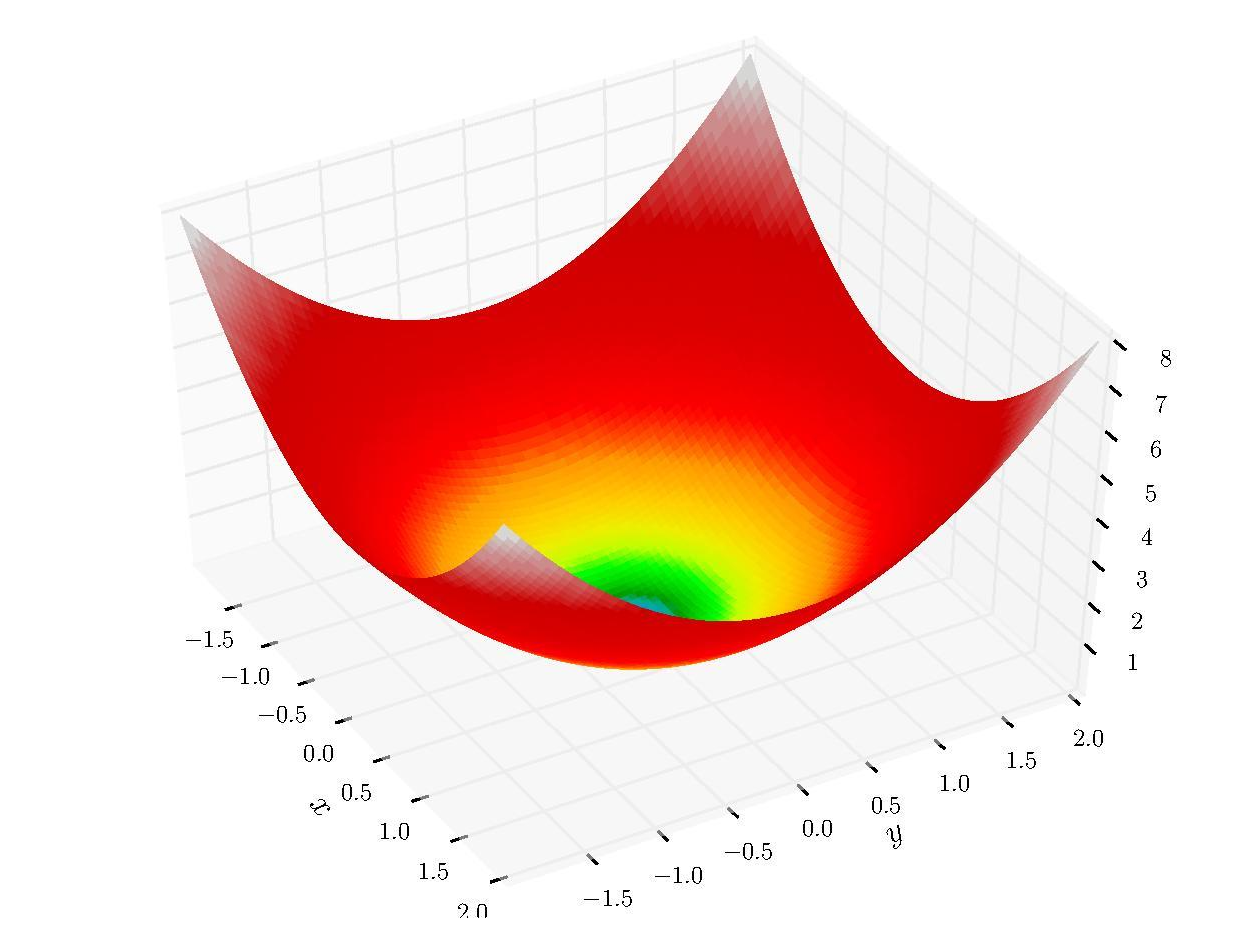
\includegraphics[width=0.9\textwidth]{sphere-function.eps}
\end{frame}

\begin{frame}
	\frametitle{Sphere function}
	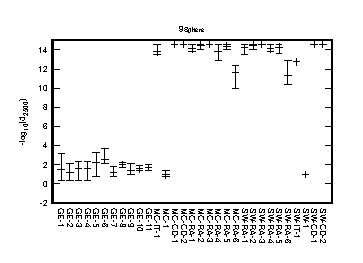
\includegraphics[width=\textwidth]{Sphere-e.eps}
\end{frame}

\begin{frame}
	\frametitle{Ackley's function}
	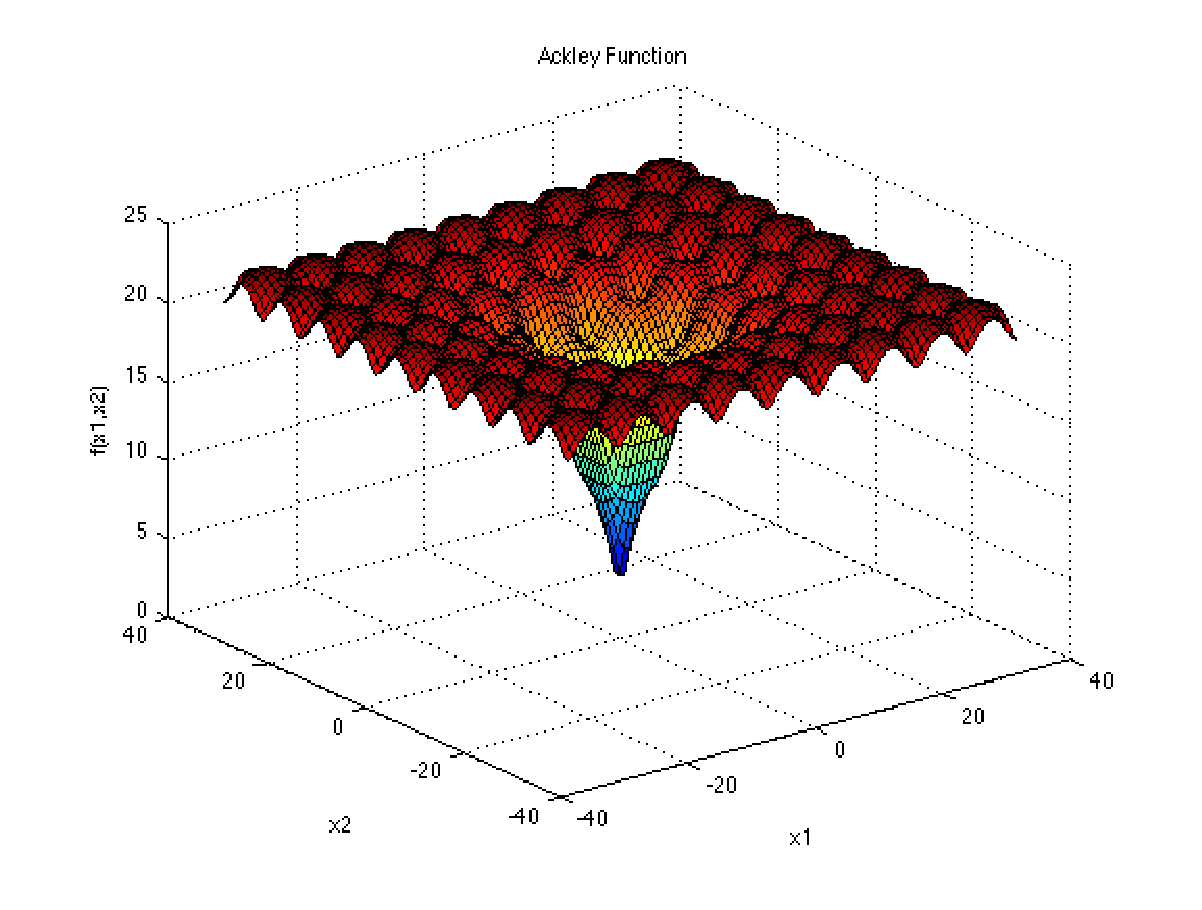
\includegraphics[width=0.9\textwidth]{ackley-function.eps}
\end{frame}

\begin{frame}
	\frametitle{Ackley's function}
	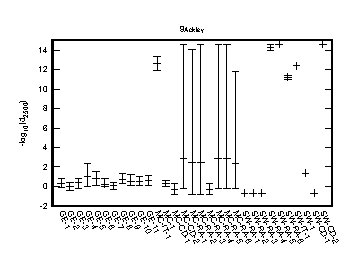
\includegraphics[width=\textwidth]{Ackley-e.eps}
\end{frame}

\begin{frame}
	\frametitle{Booth's function}
	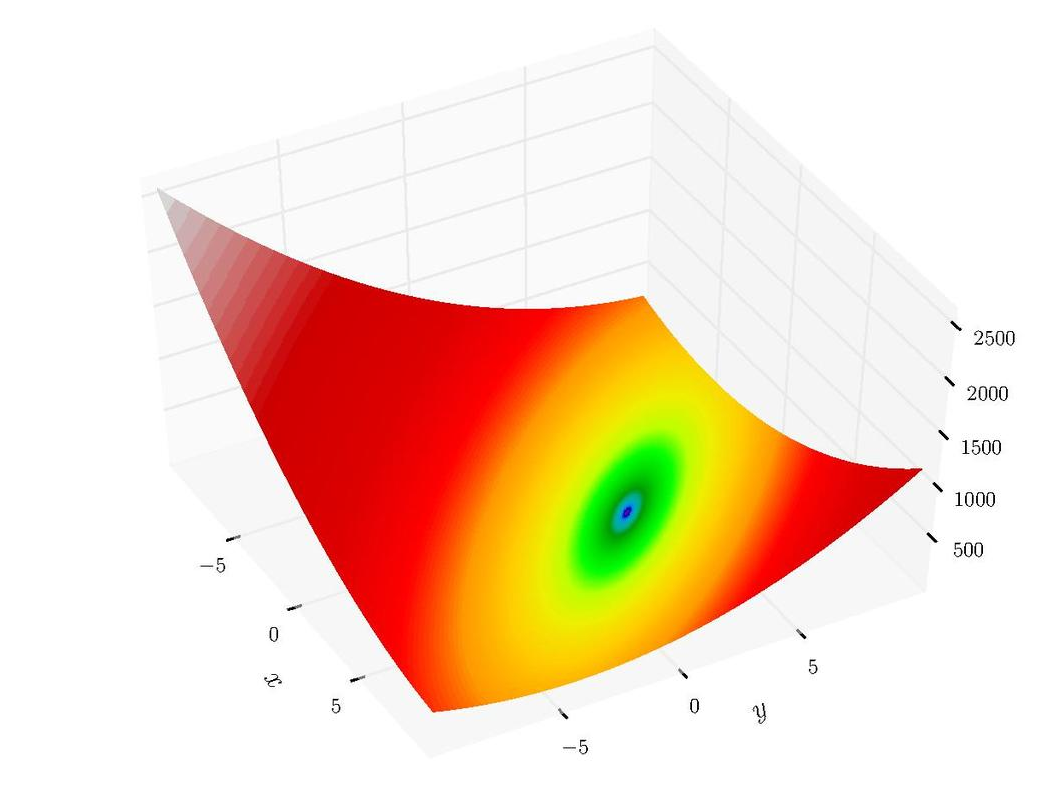
\includegraphics[width=0.9\textwidth]{booth-function.eps}
\end{frame}

\begin{frame}
	\frametitle{Booth's function}
	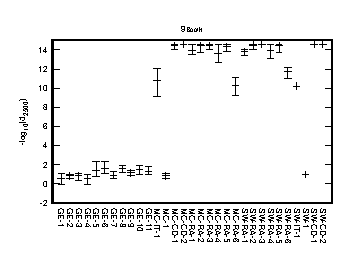
\includegraphics[width=\textwidth]{Booth-e.eps}
\end{frame}

\begin{frame}
	\frametitle{Rosenbrock's function}
	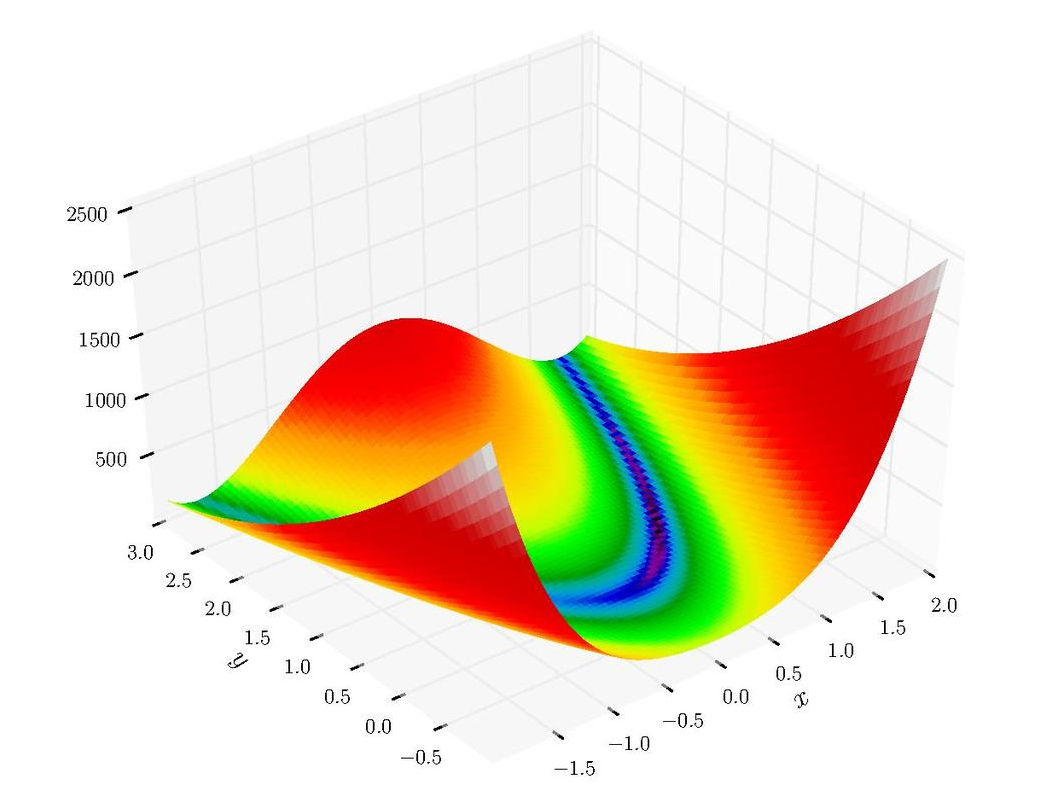
\includegraphics[width=0.9\textwidth]{rosenbrock-function.eps}
\end{frame}

\begin{frame}
	\frametitle{Rosenbrock's function}
	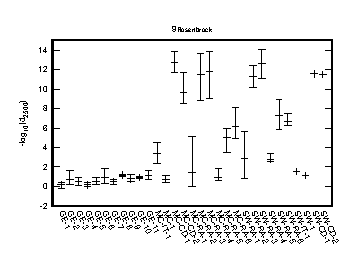
\includegraphics[width=\textwidth]{Rosenbrock-e.eps}
\end{frame}

\begin{frame}
	\frametitle{Easom's function}
	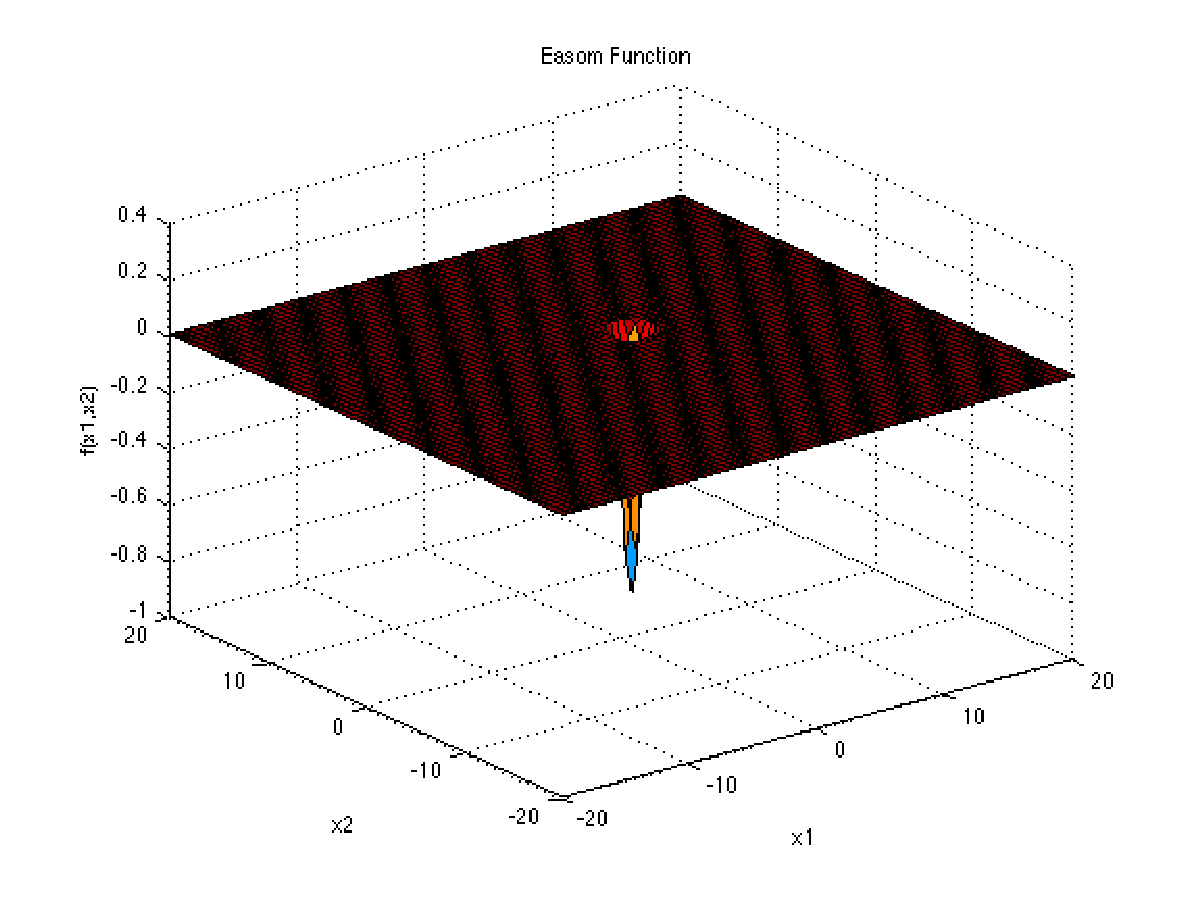
\includegraphics[width=0.9\textwidth]{easom-function.eps}
\end{frame}

\begin{frame}
	\frametitle{Easom's function}
	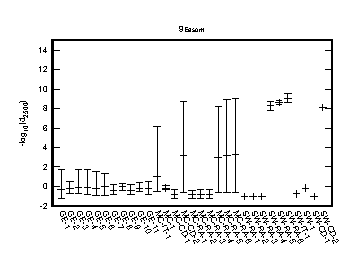
\includegraphics[width=\textwidth]{Easom-e.eps}
\end{frame}

\begin{frame}
	\frametitle{Beale's function}
	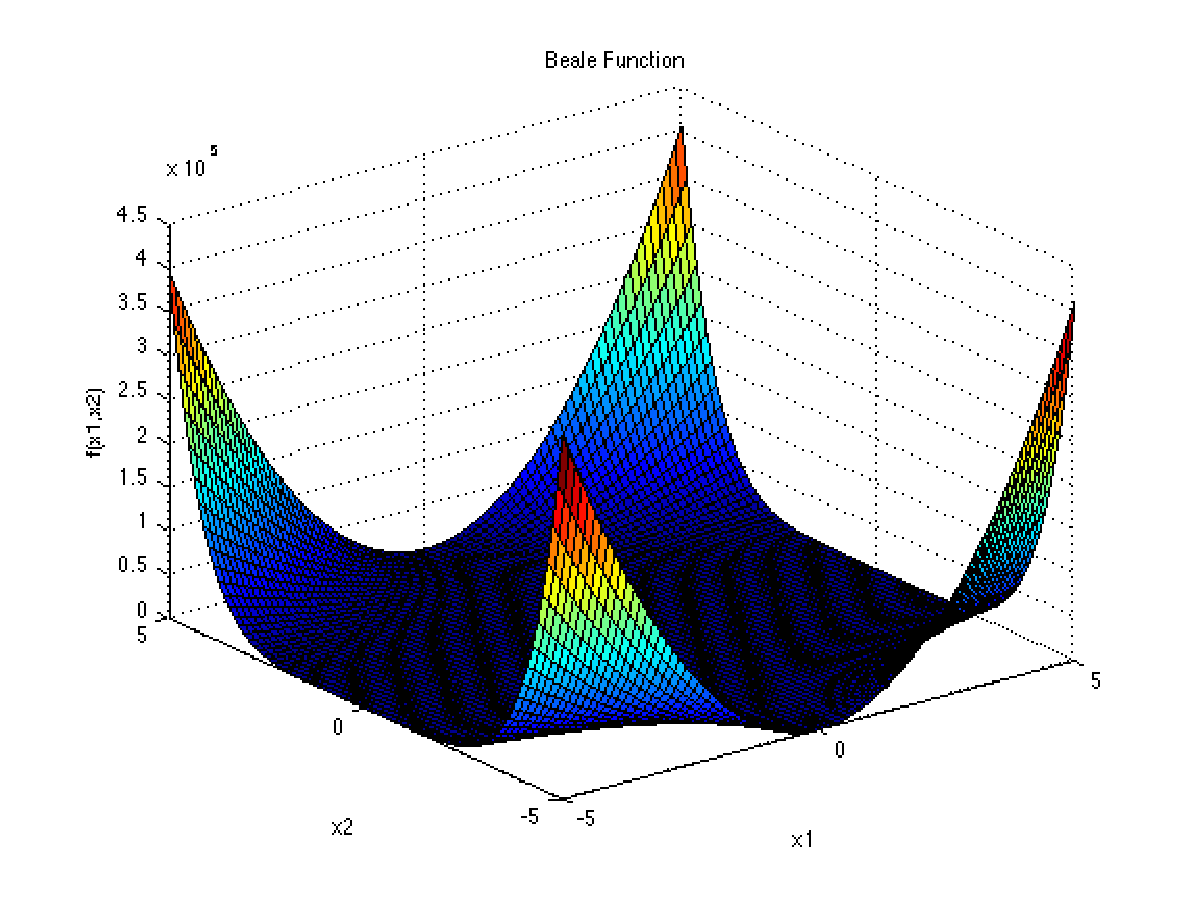
\includegraphics[width=0.9\textwidth]{beale-function.eps}
\end{frame}

\begin{frame}
	\frametitle{Beale's function}
	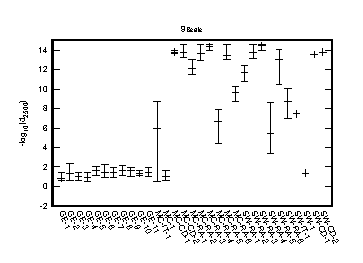
\includegraphics[width=\textwidth]{Beale-e.eps}
\end{frame}

\section{MPCOTool}

\subsection{Input files}

\begin{frame}
	\frametitle{Multi-Purposes Calibration and Optimization Tool}
	\framesubtitle{Organization}
\psset{xunit=0.4mm,yunit=0.4mm}
\PSPICTURE{-20}{-115}{260}{55}
{
	\tiny
	\rput(10,50){Main input file}
	\psframe(-20,45)(40,55)
	\psline{->}(40,50)(50,50)
	\rput(10,25){1st template file}
	\psframe(-20,20)(40,30)
	\psline{->}(40,25)(50,25)
	\psline[linestyle=dotted,dotsep=1pt]{->}(50,25)(90,25)
	\rput(10,15){$\cdots$}
	\rput(10,5){$n$-th template file}
	\psframe(-20,0)(40,10)
	\psline{->}(40,5)(50,5)
	\psline[linestyle=dotted,dotsep=1pt]{->}(50,5)(90,5)
	\rput(10,-35){$\cdots$}
	\rput(10,-75){$(N\,n)$-th template file}
	\psframe(-20,-70)(40,-80)
	\psline{->}(40,-75)(50,-75)
	\psline[linestyle=dotted,dotsep=1pt]{->}(50,-75)(90,-75)
	\rput(70,50){MPCOTool}
	\psframe(50,-95)(90,55)
	\rput(70,-110){Objective function value}
	\psframe(35,-105)(105,-115)
	\psline{->}(70,-95)(70,-105)
	\psline{->}(90,25)(100,25)
	\psline{->}(90,5)(100,5)
	\psline{->}(90,-55)(100,-55)
	\psline{->}(90,-75)(100,-75)
	\rput(120,5){$n$-th input file}
	\psframe(100,0)(140,10)
	\psline{->}(140,5)(150,5)
	\rput(120,15){$\cdots$}
	\rput(120,25){1st input file}
	\psframe(100,20)(140,30)
	\psline{->}(140,25)(145,25)(145,5)
	\rput(175,5){Simulator}
	\psframe(150,0)(200,10)
	\psline[linestyle=dashed,dash=2pt 1pt]{->}(175,10)(175,20)
	\psline[linestyle=dashed,dash=2pt 1pt]{->}(200,5)(210,7.5)
	\rput(175,25){Results file}
	\psframe[linestyle=dashed,dash=3pt 1pt](150,20)(200,30)
	\psline[linestyle=dashed,dash=2pt 1pt]{->}(200,25)(210,30)
	\rput(175,45){Experimental}
	\rput(175,40){data file}
	\psframe(150,35)(200,50)
	\psline[linestyle=dashed,dash=2pt 1pt]{->}(200,42.5)(210,30)
	\psline[linestyle=dashed,dash=2pt 1pt]{->}(150,42.5)(145,42.5)(145,25)
	\rput(230,30){Evaluator}
	\psline[linestyle=dashed,dash=2pt 1pt]{->}(230,25)(230,15)
	\psframe[linestyle=dashed,dash=3pt 1pt](210,25)(250,35)
	\rput(230,10){Objective}
	\rput(230,5){value file}
	\psframe(210,0)(250,15)
	\psline{->}(250,7.5)(260,7.5)(260,-90)(90,-90)
	\psline[linestyle=dotted,dotsep=1pt]{->}(90,-90)(70,-90)(70,-95)
	\rput(120,50){1st experiment}
	\psframe[linestyle=dotted](95,-5)(255,55)
	\rput(175,-15){$\cdots$}
	\rput(120,-75){$n$-th input file}
	\psframe(100,-80)(140,-70)
	\psline{->}(140,-75)(150,-75)
	\rput(120,-65){$\cdots$}
	\rput(120,-55){1st input file}
	\psframe(100,-60)(140,-50)
	\psline{->}(140,-55)(145,-55)(145,-75)
	\rput(175,-75){Simulator}
	\psframe(150,-80)(200,-70)
	\psline[linestyle=dashed,dash=2pt 1pt]{->}(175,-70)(175,-60)
	\psline[linestyle=dashed,dash=2pt 1pt]{->}(200,-75)(210,-72.5)
	\rput(175,-55){Results file}
	\psframe[linestyle=dashed,dash=3pt 1pt](150,-60)(200,-50)
	\psline[linestyle=dashed,dash=2pt 1pt]{->}(200,-55)(210,-50)
	\rput(175,-35){Experimental}
	\rput(175,-40){data file}
	\psframe(150,-30)(200,-45)
	\psline[linestyle=dashed,dash=2pt 1pt]{->}(200,-37.5)(210,-50)
	\psline[linestyle=dashed,dash=2pt 1pt]{->}(150,-37.5)(145,-37.5)(145,-55)
	\rput(230,-50){Evaluator}
	\psline[linestyle=dashed,dash=2pt 1pt]{->}(230,-55)(230,-65)
	\psframe[linestyle=dashed,dash=3pt 1pt](210,-55)(250,-45)
	\rput(230,-70){Objective}
	\rput(230,-75){value file}
	\psframe(210,-80)(250,-65)
	\psline(250,-72.5)(260,-72.5)
	\rput(120,-30){$N$-th experiment}
	\psframe[linestyle=dotted](95,-85)(255,-25)
}
\end{frame}

\begin{frame}
	\frametitle{Multi-Purposes Calibration and Optimization Tool}
	\framesubtitle{Error norms}
	\[L_2:\quad J=\sqrt{\sum_{i=1}^{N_{exp}}\ABS{w_i\,o_i}^2},\]
	\[L_\infty:\quad J=\max_{i=1}^{N_{exp}}\ABS{w_i\,o_i},\]
	\[L_p:\quad J=\sqrt[p]{\sum_{i=1}^{N_{exp}}\ABS{w_i\,o_i}^p},\]
	\[L_1:\quad J=\sum_{i=1}^{N_{exp}}\ABS{w_i\,o_i},\]
\end{frame}

\begin{frame}
	\frametitle{Main input file}
\psset{xunit=0.4mm,yunit=0.4mm}
\PSPICTURE{0}{-115}{280}{25}
{
	\tiny
	\psframe(0,-5)(280,25)
	\psline(40,-5)(40,25)
	\rput(20,20){\bf optimize}
	\rput(60,20){\bf simulator}
	\rput(95,20){\bf algorithm}
	\rput(130,20){evaluator}
	\rput(165,20){nsimulations}
	\rput(205,20){niterations}
	\rput(240,20){tolerance}
	\rput(265,20){nbest}
	\rput(60,10){threshold}
	\rput(95,10){npopulation}
	\rput(135,10){ngenerations}
	\rput(170,10){mutation}
	\rput(205,10){reproduction}
	\rput(240,10){adaptation}
	\rput(265,10){seed}
	\rput(60,0){direction}
	\rput(95,0){nsteps}
	\rput(130,0){nestimates}
	\rput(170,0){relaxation}
	\rput(200,0){norm}
	\rput(217,0){p}
	\rput(235,0){result}
	\rput(260,0){variables}
	\psline(20,-5)(20,-15)(40,-15)
	\psframe(40,-20)(280,-10)
	\psline(80,-20)(80,-10)
	\rput(60,-15){\bf experiment}
	\rput(95,-15){\bf name}
	\rput(125, -15){\bf template$_\mathbf{1}$}
	\rput(160,-15){template$_2$}
	\rput(195,-15){$\cdots$}
	\rput(230,-15){template$_n$}
	\rput(260,-15){weight}
	\psline(20,-15)(20,-25)
	\rput(140,-30){$\cdots$}
	\psline(20,-35)(20,-45)(40,-45)
	\psframe(40,-50)(280,-40)
	\psline(80,-50)(80,-40)
	\rput(60,-45){\bf experiment}
	\rput(95,-45){\bf name}
	\rput(125,-45){\bf template$_\mathbf{1}$}
	\rput(160,-45){template$_2$}
	\rput(195,-45){$\cdots$}
	\rput(230,-45){template$_n$}
	\rput(260,-45){weight}
	\psline(20,-45)(20,-65)(40,-65)
	\psframe(40,-75)(280,-55)
	\psline(80,-75)(80,-55)
	\rput(60,-60){\bf variable}
	\rput(95,-60){\bf name}
	\rput(120,-60){\bf minimum}
	\rput(152.5,-60){\bf maximum}
	\rput(195,-60){absolute\_minimum}
	\rput(250,-60){absolute\_maximum}
	\rput(100,-70){precision}
	\rput(130,-70){nsweeps}
	\rput(155,-70){nbits}
	\rput(175,-70){step}
	\psline(20,-65)(20,-80)
	\rput(140,-85){$\cdots$}
	\psline(20,-90)(20,-105)(40,-105)
	\psframe(40,-115)(280,-95)
	\psline(80,-115)(80,-95)
	\rput(60,-100){\bf variable}
	\rput(95,-100){\bf name}
	\rput(120,-100){\bf minimum}
	\rput(152.5,-100){\bf maximum}
	\rput(195,-100){absolute\_minimum}
	\rput(250,-100){absolute\_maximum}
	\rput(100,-110){precision}
	\rput(130,-110){nsweeps}
	\rput(155,-110){nbits}
	\rput(175,-110){step}
}
\end{frame}

\defverbatim[colored]\makeseti{
\lstset{
  language=xml,
  extendedchars=true,
  basicstyle=\tiny\ttfamily,
  showstringspaces=false,
  showspaces=false,
  tabsize=4,
  breaklines=true,
  showtabs=false,
  captionpos=b
  keywordstyle=\color{blue}\ttfamily,
  stringstyle=\color{red}\ttfamily,
}
\begin{lstlisting}[language=xml]
<optimize simulator="simulator_name" evaluator="evaluator_name"
	algorithm="algorithm_type" nsimulations="simulations_number"
	niterations="iterations_number" tolerance="tolerance_value"
	nbest="best_number" npopulation="population_number"
	ngenerations="generations_number" mutation="mutation_ratio"
	reproduction="reproduction_ratio" adaptation="adaptation_ratio"
	direction="direction_search_type" nsteps="steps_number"
	relaxation="relaxation_parameter" nestimates="estimates_number"
	threshold="threshold_parameter" norm="norm_type" p="p_parameter"
	seed="random_seed" result_file="result_file"
	variables_file="variables_file">
    <experiment name="data_file_1" template1="template_1_1"
		template2="template_1_2" ... weight="weight_1"/>
    ...
    <experiment name="data_file_N" template1="template_N_1"
		template2="template_N_2" ... weight="weight_N"/>
    <variable name="variable_1" minimum="min_value" maximum="max_value"
		precision="precision_digits" sweeps="sweeps_number"
		nbits="bits_number" step="step_size"/>
    ...
    <variable name="variable_M" minimum="min_value" maximum="max_value"
		precision="precision_digits" sweeps="sweeps_number"
		nbits="bits_number" step="step_size"/>
</optimize>
\end{lstlisting}
}

\begin{frame}
	\frametitle{Main input file: XML format}
	\makeseti
\end{frame}

\defverbatim[colored]\makesetii{
\lstset{
  language=json,
  extendedchars=true,
  basicstyle=\tiny\ttfamily,
  showstringspaces=false,
  showspaces=false,
  tabsize=4,
  breaklines=true,
  showtabs=false,
  captionpos=b
  keywordstyle=\color{green}\ttfamily,
  stringstyle=\color{red}\ttfamily,
}
\begin{lstlisting}[language=json,multicols=2]
{
	"simulator": "simulator_name",
	"evaluator": "evaluator_name",
	"algorithm": "algorithm_type",
	"nsimulations": "simulations_number",
	"niterations": "iterations_number",
	"tolerance": "tolerance_value",
	"nbest": "best_number",
	"npopulation": "population_number",
	"ngenerations": "generations_number",
	"mutation": "mutation_ratio",
	"reproduction": "reproduction_ratio",
	"adaptation": "adaptation_ratio",
	"direction": "direction_search_type",
	"nsteps": "steps_number",
	"relaxation": "relaxation_parameter",
	"nestimates": "estimates_number",
	"threshold": "threshold_parameter",
	"norm": "norm_type",
	"p": "p_parameter",
	"seed": "random_seed",
	"result_file": "result_file",
	"variables_file": "variables_file",
	"experiments":
	[
		{
			"name": "data_file_1",
			"template1": "template_1_1",
			"template2": "template_1_2",
			...
			"weight": "weight_1",
		},
	    ...
		{
			"name": "data_file_N",
			"template1": "template_N_1",
			"template2": "template_N_2",
			...
			"weight": "weight_N",
		}
	],
	"variables":
	[
		{

			"name": "variable_1",
			"minimum": "min_value",
			"maximum": "max_value",
			"precision": "precision_digits",
			"sweeps": "sweeps_number",
			"nbits": "bits_number",
			"step": "step_size",
		},
		...
		{
			"name": "variable_M",
			"minimum": "min_value",
			"maximum": "max_value",
			"precision": "precision_digits",
			"sweeps": "sweeps_number",
			"nbits": "bits_number",
			"step": "step_size",
		}
	]
}
\end{lstlisting}
}

\begin{frame}
	\frametitle{Main input file: JSON format}
	\makesetii
\end{frame}

\begin{frame}
	\frametitle {Template files}
	\begin{itemize}
		\item $N_{experiments}\times N_{inputs}$ template files are required
		\item MPCOTool parses the templates to generate the input files for
			every simulation:
		\begin{itemize}
			\item[@variableX@]: is replaced by the label associated to the
				$X$-th parameter
			\item[@valueX@]: is replaced by the value associated to the $X$-th
				parameter calculated by the optimization algorithm using the
				main input file data
		\end{itemize}
	\end{itemize}
\end{frame}

\subsection{User instructions}

\begin{frame}
	\frametitle{MPCOTool: building}
	\begin{itemize}
		\item Code in C
		\item Repository \url{https://github.com/jburguete/mpcotool}
		\item Tools required to build the executable
			\begin{itemize}
				\item C compiler: GCC or CLang
				\item Configuration tools: Automake, Autoconf and PKGConfig
				\item Control tool: GNUMake
			\end{itemize}
	\end{itemize}
\end{frame}

\begin{frame}
	\frametitle{MPCOTool: building}
	\begin{itemize}
		\item Code in C
		\item Repository \url{https://github.com/jburguete/mpcotool}
		\item Tools required to build the executable
		\item Free external libraries
		\begin{itemize}
			\item Libxml2: main input file in XML format
			\item JSON-GLib: main input file in JSON format
			\item GSL: to generate pseudo-random numbers
			\item GLib: to parse input templates and to parallelize in the CPU
				cores
			\item GTK+3: interactive graphic interface (optional)
			\item OpenMPI or MPICH: to parallelize in computer clusters
				(optional)
		\end{itemize}
	\end{itemize}
\end{frame}

\begin{frame}
	\frametitle{MPCOTool: building}
	\begin{itemize}
		\item Code in C
		\item Repository \url{https://github.com/jburguete/mpcotool}
		\item Tools required to build the executable
		\item Free external libraries
		\item Multiplatform
		\begin{itemize}
			\item Linux (Debian, Ubuntu, Fedora, OpenSUSE)
			\item Microsoft Windows (7, 8.1, 10)
			\item BSD (FreeBSD, OpenBSD, NetBSD, DragonflyBSD, Debian kFreeBSD)
			\item Illumos (Dyson, OpenIndiana)
			\item Hurd (Debian)
		\end{itemize}
	\end{itemize}
\end{frame}

\begin{frame}
	\frametitle{MPCOTool: command line}
	\begin{itemize}
		\item Running in one computer
	\end{itemize}
.$/$mpcotoolbin [-nthreads X] [-seed S] main\_input\_file.xml [results\_file]
[variables\_file]
	\begin{itemize}
		\item Parallelization in computers cluster with MPI
	\end{itemize}
mpirun [MPI options] .$/$mpcotoolbin [-nthreads X] [-seed S]
main\_input\_file.xml [results\_file] [variables\_file]
	\begin{itemize}
		\item Simulation program syntax
	\end{itemize}
.$/$simulator input\_file\_1 [input\_file\_2] [...] output\_file
	\begin{itemize}
		\item Evaluation program syntax (optional)
	\end{itemize}
.$/$evaluator simulated\_file experiment\_file results\_file
\end{frame}

\begin{frame}
	\frametitle{MPCOTool: graphic user interface application}
	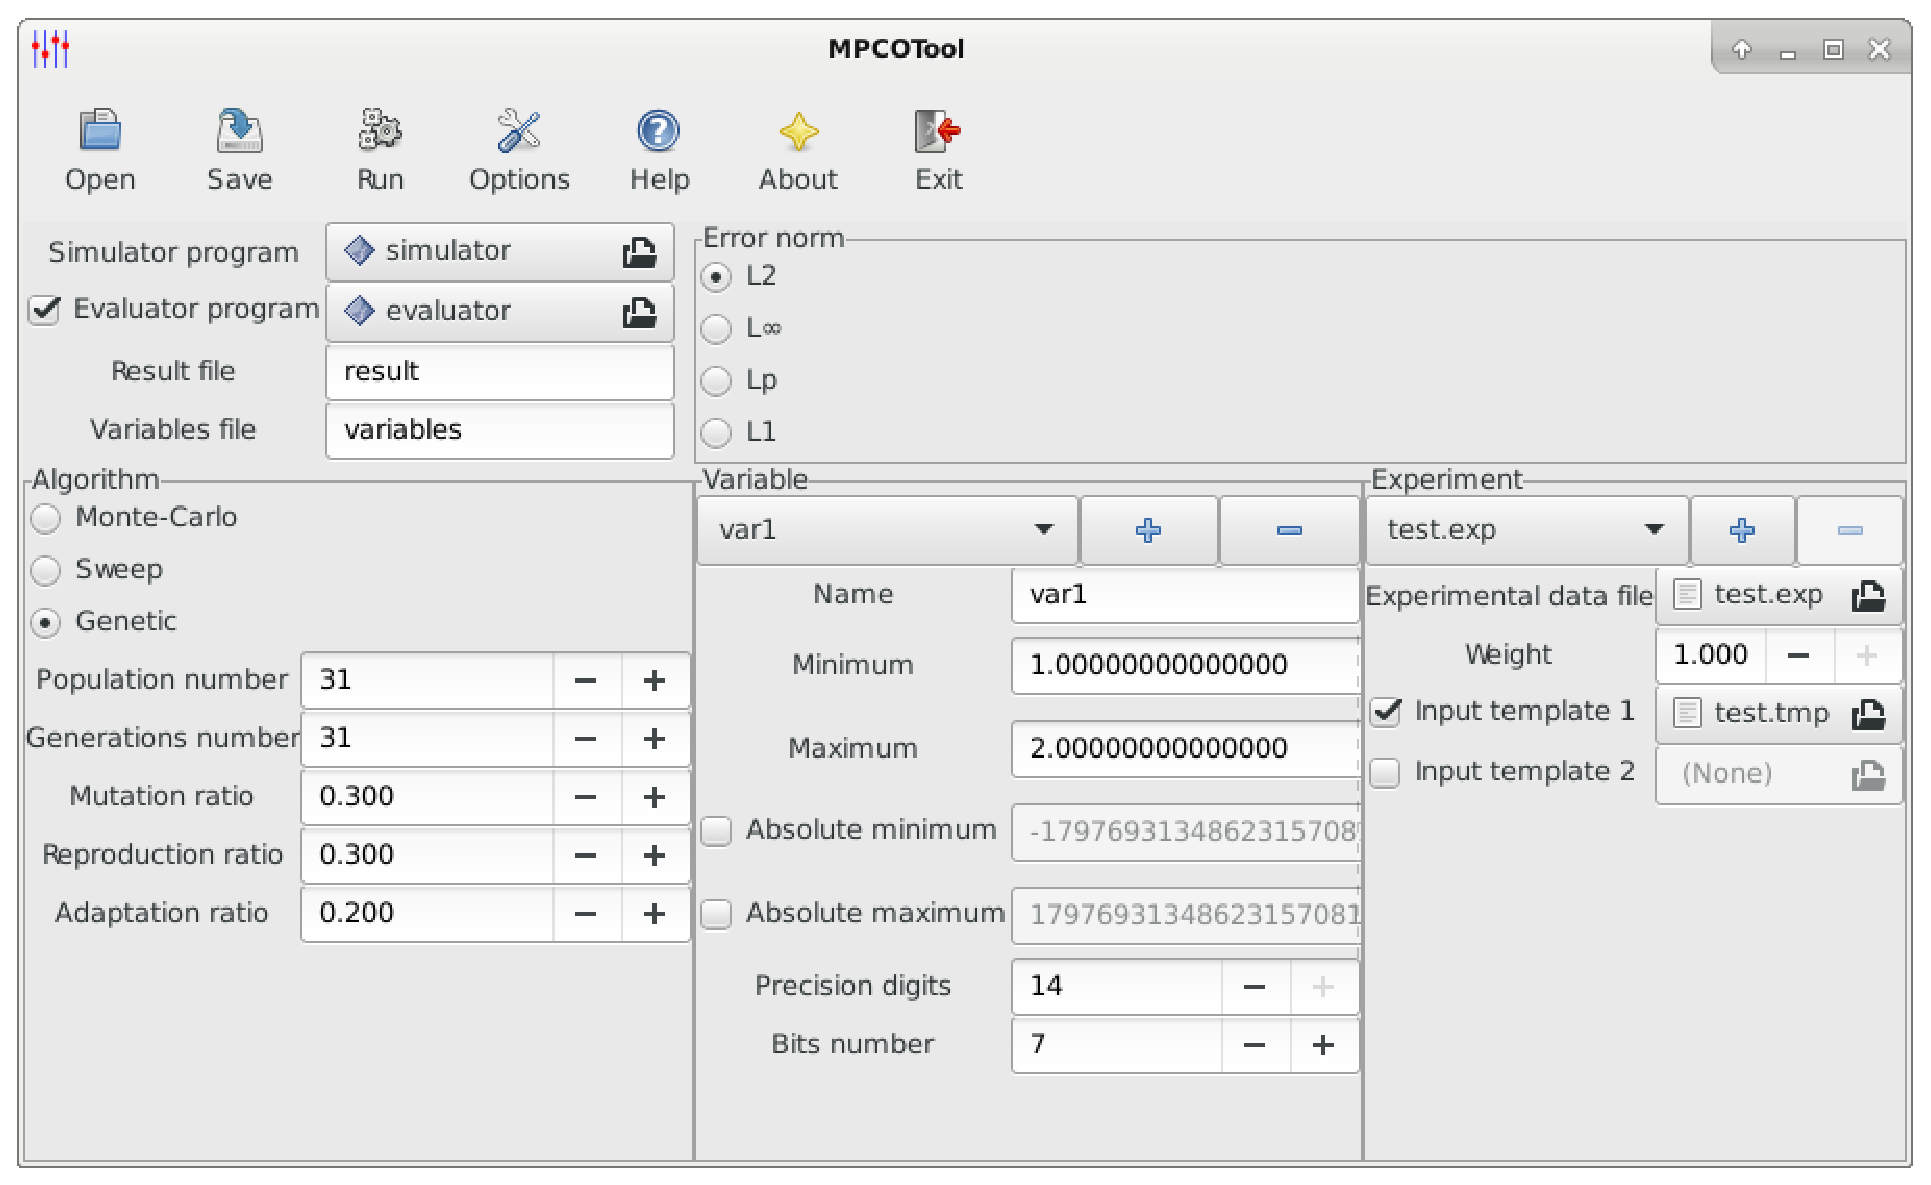
\includegraphics[width=\textwidth]{mpcotool-en.eps}
\end{frame}

\section{Practical applications}

\subsection{Optimization of gate times in a canal}

\begin{frame}
\end{frame}

\subsection{Calibration of roughness and infiltration
coefficients in furrows}

\begin{frame}
\end{frame}

\subsection{Calibration of size and friction coefficients in
sprinklers}

\begin{frame}
\end{frame}

\subsection{Calibration of movement coefficients in pivots}

\begin{frame}
\end{frame}

\section{Conclusions}

\begin{frame}
\begin{itemize}
	\item MPCOTool es una utilidad para calibración/optimización fácil,
		flexible, intuitiva, ...
	\item Implementa muchos de los algoritmos más útiles de optimización
	\item Es capaz de utilizar paralelizadamente de una forma sencilla para el
		usuario todos los recursos computacionales disponibles
\end{itemize}
\end{frame}

\begin{frame}
	\begin{center}
		\LARGE ¡GRACIAS!\\
%		\includegraphics[width=6cm]{Huerto.eps}
%		\includegraphics[width=6cm]{Vehiculo.eps}
	\end{center}
\end{frame}

\end{document}
